\documentclass[12pt,a4paper,oneside]{report}
\usepackage[utf8]{inputenc}
\usepackage[portuguese]{babel}
\usepackage[T1]{fontenc}
\usepackage{graphicx}
\usepackage{geometry}
\usepackage{url}
\usepackage{hyperref}
\usepackage{float}
\usepackage{titling}
\usepackage{fancyhdr}
\usepackage{color}
\usepackage{setspace}

% Margens
\geometry{
  a4paper,
  left=30mm,
  top=30mm,
  right=20mm,
  bottom=20mm
}

% Espaçamento
\onehalfspacing

\hypersetup{
    colorlinks=true,
    linkcolor=black,
    filecolor=black,      
    urlcolor=blue,
    titlebordercolor={1 1 1}
}

\fancyhf{}
\rfoot{\thepage}
\renewcommand{\headrulewidth}{0.4pt}
\pagestyle{fancy}

\title{
  \vspace{-2cm}
  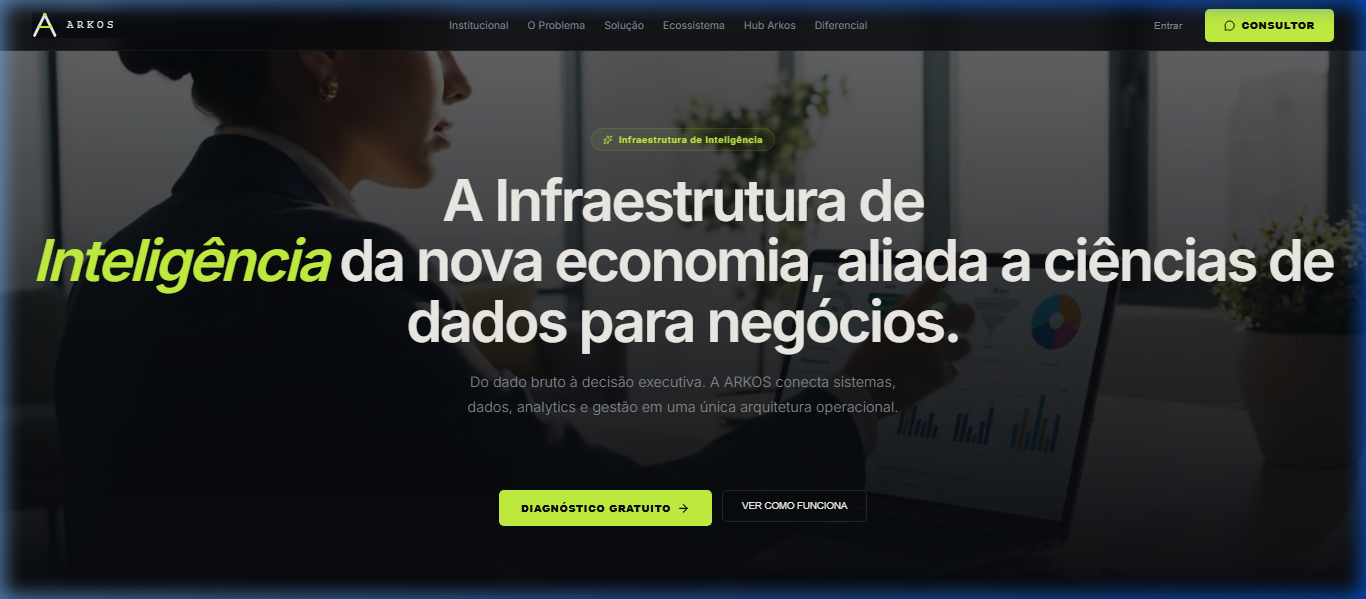
\includegraphics[width=6cm]{imagens/home_hero.png}\\[1cm]
  \textbf{RELATÓRIO INSTITUCIONAL}\\
  \large INFRAESTRUTURA DE INTELIGÊNCIA \& ECOSSISTEMA ARKOS\\
  \vspace{0.5cm}
  \large \textit{Concepção Teórica, Empresarial e Operacional}
}
\author{Arkos Intelligence}
\date{Março de 2026}

\begin{document}

\maketitle

\pagebreak
\tableofcontents
\pagebreak

% ── CAPÍTULO 1: APRESENTAÇÃO E VISÃO OPERACIONAL ─────────────────────────────
\chapter{Apresentação e Visão Operacional}

\section{Introdução}
O mercado corporativo global atravessa uma das transições mais densas da história da economia digital. A simples aquisição de softwares isolados (SaaS) ou a contratação de consultorias tradicionais já não responde à velocidade que a competitividade exige. Estruturas empresariais hoje são sufocadas por um excesso de "Silos de Informação": dados que existem, mas que não conversam entre si, impossibilitando uma tomada de decisão ágil e científica.

É nesse gargalo que se posiciona a \textbf{Arkos Intelligence}. Não vendemos softwares. Vendemos \textbf{Infraestrutura e Inteligência}. A Arkos foi idealizada como uma arquitetura operacional que integra dados, processos, auditoria e inteligência analítica em tempo real, permitindo que a administração de uma empresa transite do dado bruto diretamente para a decisão executiva auditada e automatizada.

\section{Objetivos Gerais}
A concepção deste relatório institucional visa documentar formalmente a arquitetura estrutural da Arkos para os seus co-fundadores, desenhando os marcos teóricos e as etapas de valor que o ecossistema abrange:
\begin{itemize}
  \item \textbf{Apresentar a arquitetura analítica}: Do Data Lake modular à visualização de dashboards integrados.
  \item \textbf{Demostrar a matriz estratégica}: Como o ecossistema Arkos retira gargalos operacionais e introduz economia de produtividade diária em larga escala.
  \item \textbf{Estruturar os componentes do Hub}: Módulos CLM, CRM, HRMS, ERP.
\end{itemize}

\section{A Filosofia: Infraestrutura sobre Software}
Enquanto o mercado comercializa o "Software de Prateleira" que impõe um modelo de trabalho engessado ao cliente, a Arkos desenha uma \textit{Infraestrutura de Fluxos}. 

Dizer que a Arkos vende Infraestrutura significa que implementamos a estrada por onde os dados de todas as esferas da empresa vão trafegar (Finanças, RH, Comercial, Jurídico) de forma padronizada. E a Inteligência é o motor que analisa essas interações para sugerir optimizações, disparar alertas contratuais, auditar balanços e prever fluxos de caixa com base em modelagem econométrica robusta.

\pagebreak

% ── CAPÍTULO 2: CONCEPÇÃO TEÓRICA E MESA OPERACIONAL DE DADOS ───────────────
\chapter{Concepção Teórica e Econometria de Dados}

\section{A Ciência Econômica Aplicada à Produtividade}
Nenhum painel de visualização (BI - Business Intelligence) possui utilidade se o cálculo subjacente não responder a uma lógica de causa e efeito corporativa. A matriz teórica da Arkos apoia-se fortemente nas ciências socioeconômicas e na economia aplicada.

Historicamente, o acompanhamento de metas de produtividade foca em "médias estáticas". A Arkos propõe o uso de modelagem em séries temporais e estatísticas complexas sobre o comportamento de fluxos empresariais:
\begin{itemize}
  \item \textbf{Análise de Conjuntura de Ativos}: Monitoramento inflacionário, taxa de juros e custos de insumos cruzados com despesas de contratos.
  \item \textbf{Pesquisas Quantitativas Inteligentes}: Previsão de Turnover (saída de funcionários) e funil de Recrutamento (HRMS).
  \item \textbf{Gestão de Performance Operacional}: Reengenharia de tarefas atreladas à demografia corporativa.
\end{itemize}

\begin{figure}[H]
  \centering
  % Imagem do hero da Home provando estética premium de inteligência
  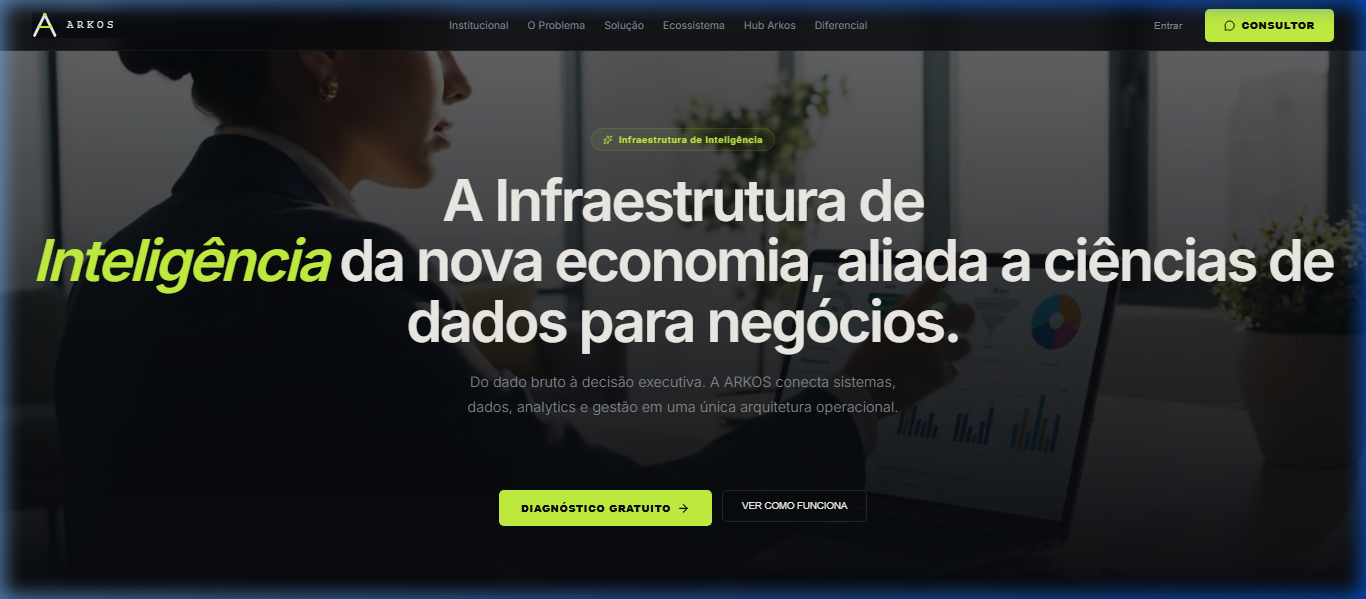
\includegraphics[width=0.85\textwidth]{imagens/home_hero.png}
  \caption{Mesa operacional da ARKOS: Visão de Infraestrutura de Inteligência para tomada de decisão executiva.}
\end{figure}

\section{A Engenharia de Performance em Larga Escala}
A performance é o dividendo que a arquitetura entrega ao C-Level da empresa. Em escala executiva, o executivo não deseja ver 10.000 linhas de planilha – ele demanda dois gatilhos: **"Onde está o erro?" e "O que fazer para corrigir?"**

O Ecossistema Arkos automatiza essa agregação. Ao conectar diretamente a base de dados centralizada do cliente à nossa esteira de fluxos:
\begin{enumerate}
    \item \textbf{Auditoria Operacional}: Detecção de inadimplementos em massa, contratos vencendo sem termo aditivo, ou duplicidades financeiras.
    \item \textbF{Predição de Gargalos}: Alerta preventivo se a velocidade do funil de vendas (CRM) não for suficiente para cobrir custos de obrigações geradas no Módulo ERP nos próximos 60 dias.
\end{enumerate}

\section{O Desafio dos Silos de Informações}
A justificativa central para a existência da Arkos reside no fato de que a maioria das corporações adota softwares isolados para cada departamento. No departamento financeiro, uma planilha. No jurídico, Word. No comercial, mensagens de texto. 

Essa desconexão de ecossistemas cria o que a literatura de gestão denomina de \textit{Silos de Ativos}. A Arkos unifica essas fontes sob um único teto operacional, permitindo que alterações no módulo de Recursos Humanos recalculem instantaneamente as projeções de folha no financeiro e o tempo de ativação de novos contratos.

\pagebreak

% ── CAPÍTULO 3: O ECOSSISTEMA ARKOS E O SEU HUB MODULAR ──────────────────────
\chapter{O Ecossistema Arkos e seu Hub Modular}

\section{O Conceito de HUB de Inteligência}
Ao realizar o login no painel central da Arkos Suite, o administrador da empresa entra em contato com o Hub completo do Ecossistema. O desenho desta interface obedece à lógica de visualização expansiva: o cliente enxerga o potencial completo das ferramentas que o Ecossistema permite entregar para a sua operação, mas opera e foca de forma destacada exclusivamente nas frentes que a empresa possui liberadas para acesso.

\section{A Estratégia de Módulos (Visualização e Liberação)}
Com o intuito de inspirar o crescimento das rotas de melhoria da empresa, os cartões de cada ferramenta no Hub apresentam uma disposição premium e informativa:
\begin{itemize}
    \item \textbf{Capas Foto-Descritivas (IA)}: Cada cartão possui uma foto coerente com a finalidade do ecossistema e uma breve descrição textual inferior.
    \item \textbf{Condição De Acesso Ativo}: Para o ecossistema ativo (atualmente Gestão de Contratos e Documentos), o cartão é destacado visualmente com contorno brilhante e transição suave ao passar o mouse.
    \item \textbf{Condição Em Desenvolvimento / Bloqueado}: Para ferramentas cujas etapas de planejamento corporativo ainda estão em andamento ou sob-contratação, uma tarja "Em Desenvolvimento" é colocada absolutamente no topo do cartão, acompanhado de opacidade reduzida para destacar o foco da empresa no ecossistema liberado.
\end{itemize}

\pagebreak

\chapter{Descrição Detalhada dos Módulos da Suíte Arkos}

\section{Introdução ao Hub de Aplicações}
A arquitetura da Arkos Suite foi projetada sobre um modelo de microsserviços integrados de alta densidade. O ecossistema é composto por plataformas modulares que atuam em simbiose para desatar os gargalos operacionais e escalar a inteligência de negócios.

Garantimos que cada plataforma possua seu próprio motor analítico:

\subsection{Módulo 1: Marketing Intelligence (Inteligência de Mercado)}
O marketing atua como gerador supremo de dados decisórios. Operamos desde o digital analítico até a inteligência profunda, pesquisas quantitativas e qualitativas de mercado, NPS, testes de lançamentos e preços, monitoramento de menções e análise de sentimento nas redes sociais. Tudo convertido em inteligência para a sua tomada de decisão.

\subsection{Módulo 2: Arkos Data (Infraestrutura de Dados)}
Data warehouse, APIs, pipelines e governança de dados. Criamos uma central única que organiza todas as informações da sua empresa, eliminando planilhas soltas e garantido que a diretoria tome decisões baseada em números reais, e não em achismos.

\subsection{Módulo 3: Arkos CRM (Gestão de Relacionamento e Conversão)}
\textbf{Objetivo}: Analisar e escalar a eficiência do funil de conversão comercial da corporação através de ciência de dados.
\begin{itemize}
    \item \textbf{Visão em Tempo Real}: Acompanhamento instantâneo da esteira de leads, interações de atendimento e taxa de fechamento.
    \item \textbf{Cálculo Automatizado de Custos de Vendas (CAC e LTV)}: Permite saber em tempo real o Custo de Aquisição de Cliente (CAC) e o Retorno Financeiro dele ao longo do tempo (LTV). Cruzamos investimentos de captação direto com contratos consolidados, permitindo prever o lucro real por canal de venda.
    \item \textbf{Integração Cross-Sector}: Alerta automático à operação se o fluxo de fechamento demandar aumento imediato de suprimentos no faturamento (ERP) ou contratação de pessoal (Recursos Humanos).
\end{itemize}

\subsection{Módulo 4: Arkos ERP (Gestão de Finanças em Tempo Real)}
\textbf{Objetivo}: Consolidar o motor financeiro e controle operacional em tempo real atrelado a modelagens econométricas preventivas.
\begin{itemize}
    \item \textbf{Fluxo de Caixa Dinâmico}: Toda movimentação, emissão de faturas, contratos vigentes e pedidos de fornecedores são sintetizados instantaneamente para o C-Level.
    \item \textbf{Gestão de Fornecedores e Tickets}: Controle rígido de ordens de compra e fluxos de pagamentos linked a contratos auditáveis, prevenindo vazamentos de capital.
    \item \textbf{Projeções Estatísticas (GPS Financeiro)}: Em vez de registrar o que já foi gasto, o ERP da Arkos faz projeções econométricas alertando se os custos de outros setores superarão as receitas previstas para os próximos 60 dias.
\end{itemize}

\subsection{Módulo 5: Arkos AI Agents (Agentes de IA)}
Agentes autônomos treinados com as regras específicas do seu negócio para resolver chamados e triagens complexas diretamente via canais de atendimento (WhatsApp/Web), reduzindo drasticamente custos de suporte.

\subsection{Módulo 6: Arkos Commerce \& SaaS (Motor de Vendas)}
Motor financeiro robusto 100\% integrado à gestão executiva para e-commerce, recorrência, subscrições de produtos/mensalidades e integrações bancárias diretas automatizadas.

\subsection{Módulo 7: Arkos Growth Agency (Escalabilidade de Marca)}
Squads avançados para empresas parceiras operando desenvolvimento web, landing pages exclusivas, tráfego pago altamente parametrizado e produção audiovisual de marca.

\subsection{Módulo 8: Arkos Strategy Planner (Planejamento Estratégico)}
Formulação e acompanhamento de planejamento estrutural. Oferecemos um sistema autônomo visual que orienta todos os passos, desde a identidade organizacional até a operação tática, ou via consultoria especializada.

\subsection{Módulo 9: Arkos Academy (LMS / EdTech)}
Plataforma de ensino dupla. Internamente, treina e atualiza clientes e líderes em dados e economia competitiva. Externamente, atua como Portal EAD completo para faculdades e escolas, acoplando diagnóstico e predição discente.

\subsection{Módulo 10: Arkos IT \& Infra (Gestão de TI)}
Gestão compartilhada de TI a distância. Atuamos como seu departamento de ponta, elevando a eficiência de empresas com setores legados. Cuidamos da segurança de servidores à administração web.

\subsection{Módulo 11: Arkos Recursos Humanos}
Triagem automatizada de currículos assistida por ferramentas de IA. Executa rankeamento e dossiê de candidatos, gestão de DP (folha de pagamento) e KPIs de capital humano calibrados ao faturamento executivo.

\begin{figure}[H]
  \centering
  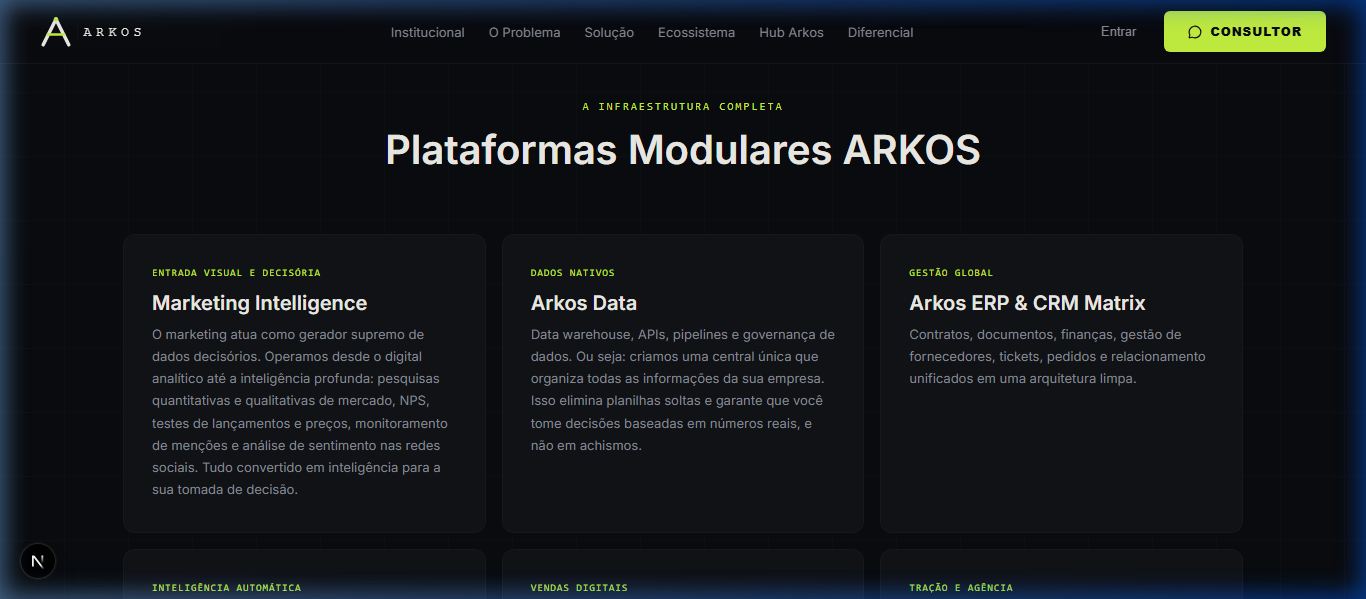
\includegraphics[width=0.85\textwidth]{imagens/hub_modulos_lista.png}
  \caption{Visão expandida da Suite Arkos: 11 Plataformas modulares desenhadas para agir em simbiose operacional contínua.}
\end{figure}

\section{Nossos Diferenciais Competitivos}
A Arkos não compete com softwares isolados (SaaS de Prateleira). Nossa proposta diferencia-se por entregar \textbf{Infraestrutura e Inteligência Ativa}:
\begin{itemize}
    \item \textbf{Operação Analítica de Alto Nível}: Cruzamento de dados cross-módulos com validação em tempo real. Menos de 5\% das empresas conseguem esse nível de assertividade econométrica sem terceirizar BIs manuais.
    \item \textbf{Letramento Nativo de Equipe}: Os algoritmos preditivos e dashboards são construídos para dar \textbf{autonomia decisória} à corporação parceira de forma independente.
    \item \textbf{Arquitetura em 4 Camadas}: Processamento seguro desde a ingestão passiva de Fontes Isoladas (ERP, planilhas), passando pelo \textbf{Data Lake Node} (ETL), Processamento de Predictive Analytics até a ponta da interface rodando inteligência natural.
\end{itemize}

\begin{figure}[H]
  \centering
  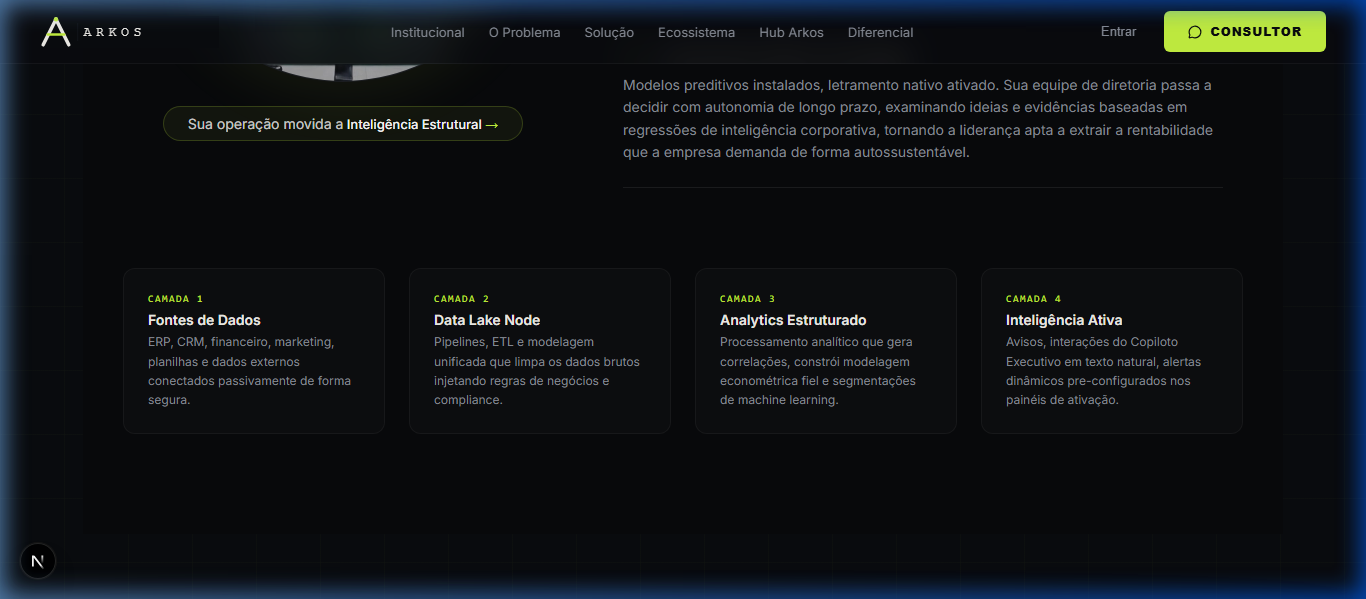
\includegraphics[width=0.85\textwidth]{imagens/diferenciais.png}
  \caption{Mesa operacional da @ARKOS: Operação Analítica de Alto Nível de Infraestrutura.}
\end{figure}

\section{Ferramentas de Suporte Nativas (.Micro-Apps)}
Além das plataformas matriciais de gestão, a Workspace da Arkos fornece em sua malha interna aplicativos focados em produtividade e colaboração unificada:
\begin{itemize}
    \item \textbf{Arkos Cloud}: Buffer seguro para classificar e auditar mídias e entregáveis documentais.
    \item \textbf{Arkos Rooms}: Reuniões remotas com transcrição IA e auto-geração de Atas em PDF direto para o financeiro ou CLM.
    \item \textbf{Arkos Flow}: Painéis Scrum e Kanban nativos para gestão ágil de projetos por setor em tempo real.
    \item \textbf{Arkos Connect}: Feed corporativo interno para rituais e avisos com total confidencialidade.
    \item \textbf{Arkos LiveTranslate & SmartBooking}: Agendamentos vinculados a disparos de WhatsApp e pontes de tradução para ligações globais.
\end{itemize}

\begin{figure}[H]
  \centering
  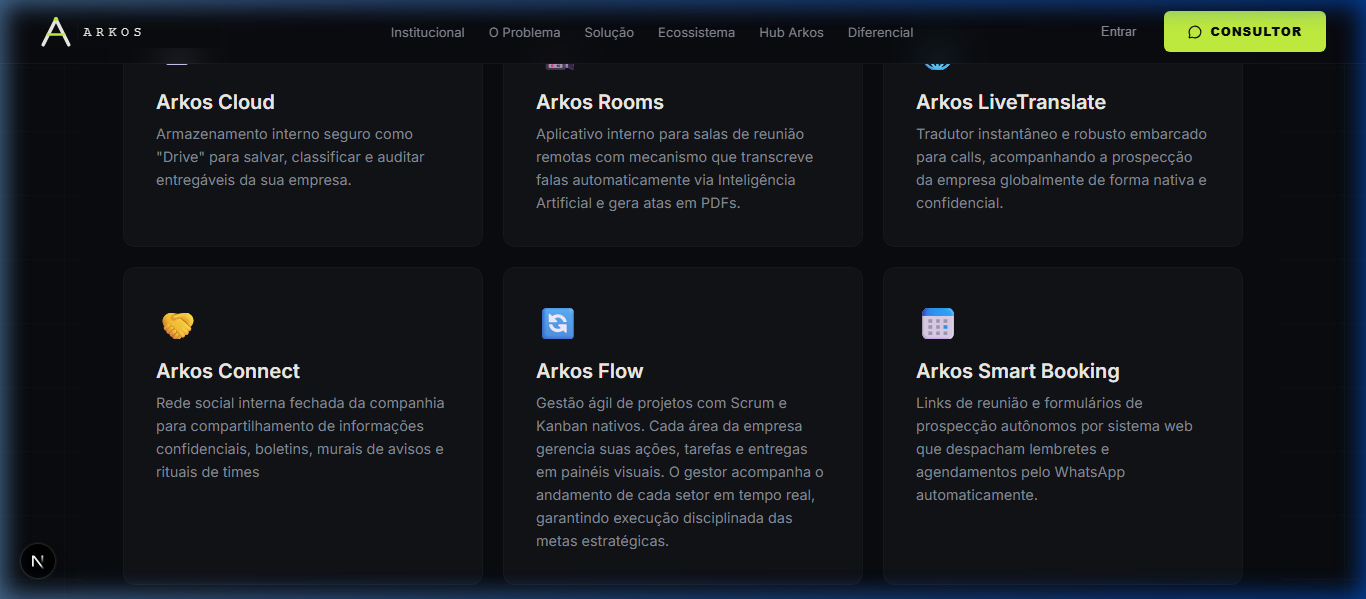
\includegraphics[width=0.85\textwidth]{imagens/micro_apps_grid.png}
  \caption{Hub de Aplicações de Micro-Apps nativos prontas para a rotina executiva.}
\end{figure}

\pagebreak

\pagebreak
\chapter{Metodologia de Implantação e Governança}

\section{O Framework de Ativação Arkos}
A implementação de uma Infraestrutura de Inteligência não ocorre do dia para a noite. Ela segue um framework estruturado para garantir que a transição dos sistemas legados do cliente para o Ecossistema Arkos ocorra sem fricção operacional e com integridade total de dados.

O processo é dividido em quatro fases cíclicas de valorização:

\subsection{Fase 1: Diagnóstico e Mapeamento de Silos (Assessment)}
Antes de conectar qualquer dado, a equipe de cientistas e economistas da Arkos realiza uma varredura das fontes de informação do cliente.
\begin{itemize}
    \item Identificação de planilhas isoladas, contratos físicos e softwares terceiros.
    \item Definição de métricas de sucesso (KPIs e OKRs) que o C-Level deseja monitorar no dashboard ativo.
    \item Mapeamento de Gargalos de Auditoria: Onde estão ocorrendo vazamentos de capital ou retrabalho?
\end{itemize}

\subsection{Fase 2: Ingestão de Dados e ETL (Data Lake Ingestion)}
Nesta fase, constrói-se a "esteira de dados". Os registros legados são extraídos, tratados, limpos e injetados na infraestrutura segura da Arkos.
\begin{itemize}
    \item Padronização de modelos de dados (ex: unificar cadastros de clientes dispersos).
    \item Upload de documentos históricos no repositório seguro para processamento analítico (OCR).
    \item Homologação de tokens e chaves de API para integrações ao vivo.
\end{itemize}

\subsection{Fase 3: Parametrização e Ativação de Módulos (Rollout)}
Os módulos contratados (como o módulo CLM de Contratos) são calibrados conforme as regras de negócio da empresa corporativa parceira:
\begin{itemize}
    \item Definição de permissões de acesso por perfil (Segurança de Pessoal).
    \item Criação de templates de minuta e automação de variáveis.
    \item Testes de estresse de fluxos de assinatura e aprovação digital.
\end{itemize}

\subsection{Fase 4: Expansão Analítica (Scale Up)}
Uma vez que o módulo prioritário está rodando fluentemente, a Arkos inicia a inteligência cruzada. Dados acumulados de 30 a 60 dias de operação começam a gerar os primeiros insights preditivos, acionando as modelagens econométricas para sugestões de otimização de custos e refinamento de forecast de receitas.

\section{Governança e Segurança da Informação}
Dado que a Arkos manipula ecossistemas de dados estratégicos e contratuais, a segurança é posicionada na base da pirâmide arquitetural:
\begin{itemize}
    \item \textbf{Criptografia em Trânsito e Repouso}: Garantia de que nenhum dado seja interceptado.
    \item \textbf{Segregação de Tenancy (Multi-tenant seguro)}: Dados de uma empresa nunca interagem ou residem em canais compartilhados de memória com dados de outra corporação.
    \item \textbf{Audit Trail Absoluto}: O registro de quem acessou, modificou ou visualizou qualquer registro garante conformidade com as melhores práticas de compliance e segurança digitais.
\end{itemize}

\pagebreak
\chapter{Considerações Finais e Próximos Passos}

\section{Conclusão da Visão de Ecossistema}
A Arkos Intelligence posiciona-se não como um fornecedor, mas como um \textbf{Parceiro Estratégico de Infraestrutura}. A unificação dos módulos de Contratos, Comercial, RH e Operações sob um único motor econométrico auditável retira a empresa da "névoa de dados" e a lança em um patamar de gestão científica.

\section{Próximas Etapas (Próximos 60 Dias)}
Para consolidar o crescimento e estabilidade do ecossistema para os co-criadores e primeiros parceiros corporativos:
\begin{itemize}
    \item \textbf{Consolidação Total do Módulo CLM}: Estabilização de fluxos massivos de assinatura e automações de reajustes.
    \item \textbf{Auditório de Moodle/LMS}: Integração de dados de performance acadêmica e treinamento corporativo se aplicável.
    \item \textbf{Refinamento de UX/UI dos Módulos Bloqueados}: Garantir o gatilho visual do Hub para incentivar cross-selling e ativações graduais.
\end{itemize}

\vspace{2cm}
\begin{center}
    \rule{8cm}{0.4pt}\\
    \small \textbf{ARKOS INTELLIGENCE}\\
    \large \textit{"Do dado bruto à decisão executiva."}
\end{center}

\pagebreak


\end{document}
